All further reservoirs were constructed with the parameters from this baseline,
unless otherwise specified. The default reservoir size used was 200 hidden
nodes. $\mathbf{W}^{res}$ and $\mathbf{W}^{in}$ were both generated as random
matrices with i.i.d. entries in the interval [-0.5, 0.5]. Both matrices are
fully connected, and the reservoir weight matrix was rescaled such that
$\rho(\mathbf{W}_{res}) = 0.9$. The first 200 states of each run are discarded
to provide a \textit{washout} of the initial reservoir state. For all
experiments, the generated input was split into a training and test set, with
$L_{train} = 2000$ and $L_{test} = 3000$. All reported performances are the mean
across ten randomizations of each model representative. The Python software
library implementation is available online\footnote{Some GitHub repository.}.

\subsection{Noise}

We model AWGN noise by extending the ESN model to take the sum of two individual
inputs, $u$ and $v$, which represent the signal and the noise. The goal of the
reservoir remains a computation on the signal $u$, a task now hindered by the
unwanted noise.

We vary the signal to noise ratio of the injected noise when running the test
dataset. Thus we will see the inherent robustness of the reservoirs to undesired
noise that is previously unseen. The results are shown in
Fig. \ref{input_noise_snr}, illustrating a slight performance degradation when
the ratio of signal power to noise power drops below 20 dB. The reservoir
performance drops more drastically when reaching 10 dB. Similar performance
degradation was seen in \cite{dambre_information_2012}, where the same SNR
measure was used to evaluate the signal reconstruction capacity from the state
of a dynamical system.

\begin{figure}
  \centering
  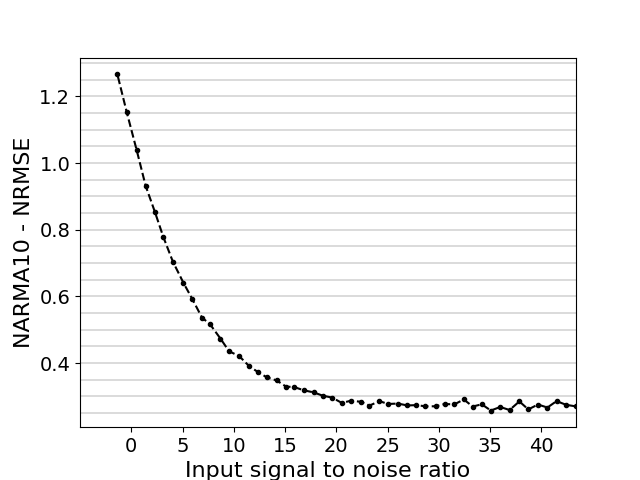
\includegraphics[width=2.5in]{img/input_noise_snr.png}
  \caption{
    Noise causing a decrease in performance of a reservoir with 200 hidden nodes
on the NARMA10 task. Input signal to noise ratio is measured in dB, and is
calculated as $SNR = 10\log_{10}(\frac{var(u)}{var(v)})$, the measure also used
in \cite{dambre_information_2012}.
  }
  \label{input_noise_snr}
\end{figure}

%%% Local Variables:
%%% mode: latex
%%% TeX-master: "../main"
%%% End:
